\documentclass{beamer}
\usepackage[italian]{babel}
\usepackage{graphicx}
\usepackage{bm}
\usepackage{listings}
\usepackage{hyperref}
\usepackage{hyperref}
\usepackage[italian]{babel}
\RequirePackage{palatino}
\RequirePackage[utf8]{inputenc}
\RequirePackage[T1]{fontenc}

\usefonttheme{serif}
\graphicspath{ {./pic/} }

\definecolor{primary}{HTML}{977478}
\definecolor{secondary}{HTML}{747897}
\definecolor{tertiary}{HTML}{789774}

\lstdefinestyle{mystyle}{
    commentstyle=\bfseries\color{tertiary},
    keywordstyle=\bfseries\color{secondary},
    numberstyle=\tiny\color{secondary},
    stringstyle=\color{secondary},
    basicstyle=\ttfamily\footnotesize,
    breakatwhitespace=false,         
    breaklines=true,                 
    captionpos=b,                    
    keepspaces=true,                 
    numbers=left,                    
    numbersep=5pt,                  
    showspaces=false,                
    showstringspaces=false,
    showtabs=false,                  
    tabsize=2,
    morekeywords={include,inductive,Term,type,z,prod,Univ,let,rec,on,match,with},
    morecomment=[l]{\#},
    mathescape=true
}

\lstset{style=mystyle}

\newcommand{\makepart}[1]{ % For convenience
\part{#1} \frame{
  \partpage}
}

\newcommand{\makesection}[1]{
  \section{#1}
  \setbeamercolor{alerted text}{fg=primary}
  \fontsize{21pt}{7.2}\selectfont
  \begin{frame}{\ }
    \alert{#1}
  \end{frame}
  \fontsize{12pt}{15}\selectfont
  \setbeamercolor{alerted text}{fg=secondary}
}

\usepackage{styles/elegantmacros}
\usepackage{styles/bussproofs}
\usefolder{styles}
\usetheme[style=blue]{elegant}


\setlength{\itemsep}{50.mm}


\title[
]{Da Matita a Dedukti e ritorno}

\subtitle{sottotitolo che non so ancora cosa}

\author[
]{
    Mattia Girolimetto
}

\institute{
Relazione per il corso 85001 - Metodi logici per la Filosofia \\
    Alma Mater Studiorum, Università di Bologna}
\date{19 Luglio 2023}

\begin{document}
\begin{frame}
  \titlepage
\end{frame}

\begin{frame}{Indice}
  \tableofcontents[]
\end{frame}


\makesection{Dedukti e Matita}

\subsection{I proof assistant}
\begin{frame}{I proof assistant}
\begin{center}

\includegraphics[scale=0.5]{proofAssistant.png}
\end{center}
\end{frame}
\begin{frame}{Isomorfismo di Curry-Howard}
\begin{center}
  \begin{tabular}{ c  c  c }
    \textbf{\alert{LOGICA}} &  & \textbf{\alert{TEORIA DEI TIPI}} \\ \\
    Proposizioni & $\Leftrightarrow$ & Tipi \\ \\
    Dimostrazioni & $\Leftrightarrow$ & Programmi \\ \\
    Verifica di una dimostrazione & $\Leftrightarrow$ & Verifica di tipo \\ \\
  \end{tabular}
\end{center}
\end{frame}

\begin{frame}{I proof assistant}
  \begin{center}
    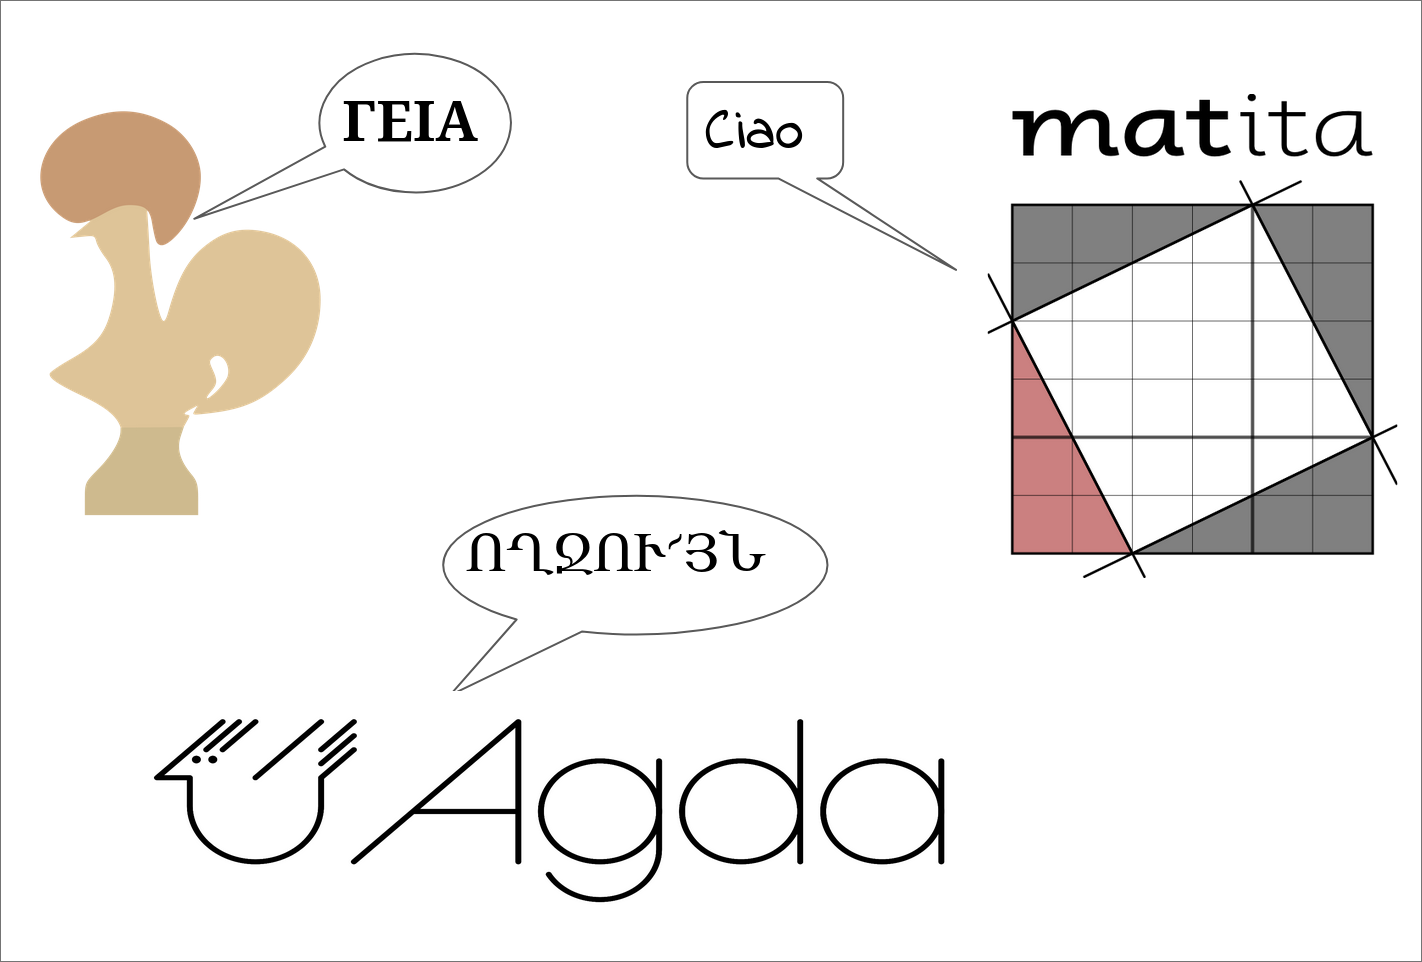
\includegraphics[scale=0.25]{inter.png}
  \end{center}
\end{frame}

\subsection{Dedukti}
\begin{frame}{Dedukti}
\begin{columns}

\begin{column}{.5\textwidth}
\begin{itemize}
  \item Framework logico
  \vspace{1.5em}
  \item Implementa logiche e teoremi
  \vspace{1.5em}
  \item Basato sul $\lambda\Pi$-calcolo modulo
\end{itemize}
\end{column}

\begin{column}{.5\textwidth}

\includegraphics[scale=1]{dedukti2.png}
\end{column}
\end{columns}
\end{frame}

\begin{frame}{$\lambda\Pi$-calcolo modulo}
  Estende il \textit{$\lambda$-calcolo tipizzato} aggiungendo
\begin{itemize}
  \vspace{1em}
  \item Tipi dipendenti 
  \vspace{1em}
  \item Regole di riscrittura
\end{itemize}
\pause
\begin{exampleblock}{Esempio (Regole di riscrittura)}
\begin{center}
  $sum$ $n$ $0$ $\hookrightarrow$ $n$ \\
  \vspace{1em}
  $prod $ $n$ $0$ $\hookrightarrow$ $0$
\end{center}
\end{exampleblock}
\end{frame}

\subsection{Matita}
\begin{frame}{Matita}
\begin{columns}
  \begin{column}{.5\textwidth}
    \begin{itemize}
      \item Proof assistant sviluppato all'Università di Bologna
      \vspace{1.5em}
      \item Basato sul calcolo delle \textit{costruzioni (co)induttive}
    \end{itemize}
  \end{column}
  \begin{column}{.5\textwidth}
    \begin{center}
        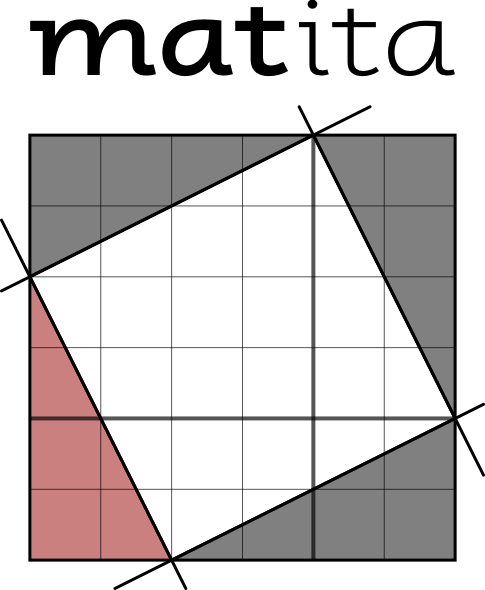
\includegraphics[scale=0.30]{matita.png}
    \end{center}
  \end{column}
\end{columns}
\end{frame}

\begin{frame}[fragile]{Calcolo delle costruzioni (co)induttive}
Caratteriazzato dalla possibilità di definire 
\begin{itemize}
  \item \textit{tipi induttivi}
  \item \textit{punto fissi}
  \item \textit{pattern matching}
\end{itemize}

\begin{center}
  \begin{lstlisting}[numbers=none]
inductive nat: Type[0] $\stackrel{\text{def}}{=}$
   O : nat
 | S : nat $\rightarrow$ nat.

let rec plus n m on n $\stackrel{\text{def}}{=}$
 match n with
 [ O $\Rightarrow$ m
 | S x $\Rightarrow$ S (plus x m)
 ].
\end{lstlisting}
\end{center}

\end{frame}

\makesection{Esportazione}
\subsection{Krajono}
\begin{frame}{Krajono}

\begin{columns}
\begin{column}{.5\textwidth}
\begin{itemize}
  \item \textit{Fork } di Matita 
  \vspace{1.5em}
  \item Aggiunge l'esportazione verso Dedukti
  \vspace{1.5em}
  \item Non più supportato
\end{itemize}
\end{column}
\begin{column}{.5\textwidth}

\includegraphics[scale=0.40]{m2d.png}
\end{column}
\end{columns}

\end{frame}

\subsection{La codifica}
\begin{frame}{La codifica}
  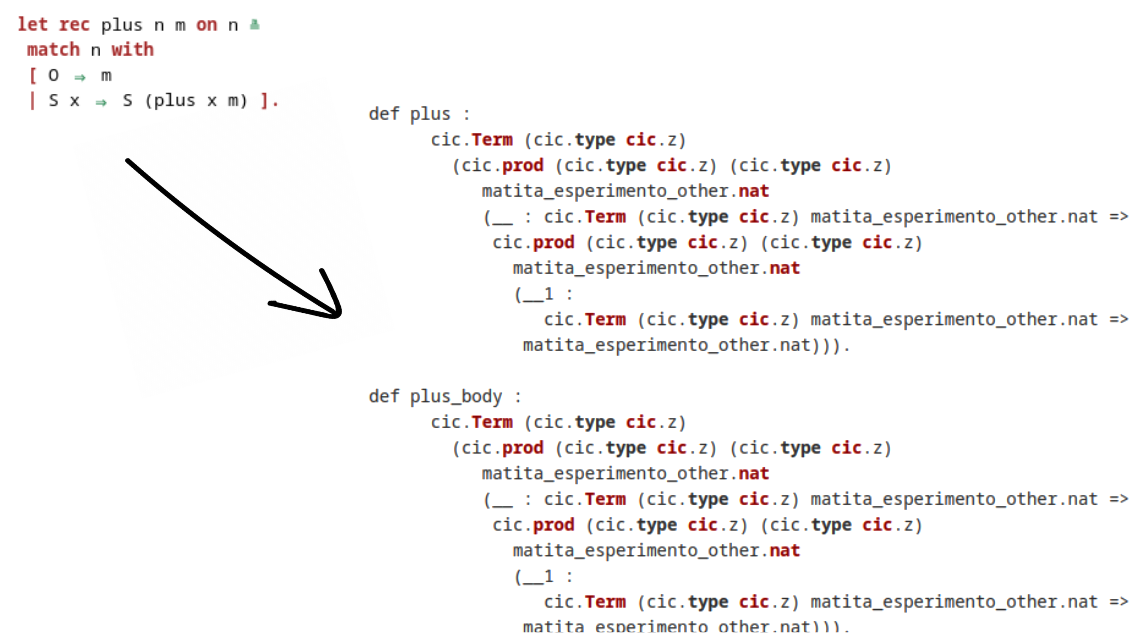
\includegraphics[scale=0.40]{export.png}
\end{frame}

\makesection{Importazione}
\begin{frame}
  \begin{center}
    
\includegraphics[scale=0.50]{m2d2m.png}
  \end{center}
\end{frame}

\subsection{Problemi}
\begin{frame}{Problemi}
\begin{itemize}
  \item \alert{\textbf{Problema}} In Dedukti le proprietà di \textit{confluenza} e 
    \textit{normalizzazione} non sono garantite.
\end{itemize}
\end{frame}

\begin{frame}{Confluenza e normalizzazione}
  \begin{block}{Definizione (Confluenza)} 
    Dato un termine $a$, se esistono due regole di riscrittura $a \hookrightarrow^* b$ e 
    $a \hookrightarrow^*c$, allora esiste un termine $d$ tale che $b \hookrightarrow^* d$
    e $c \hookrightarrow^* d$.
  \end{block}
  \begin{center}
    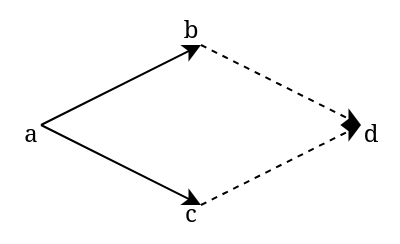
\includegraphics[scale=0.40]{confluenza.png}
  \end{center}
  \begin{block}{Definizione (Normalizzazione)} 
    Dato un termine, questo può essere ridotto al più un numero finito di volte.
  \end{block}
\end{frame}

\begin{frame}{Problemi}
\begin{itemize}
  \item \alert{\textbf{Problema}} In Dedukti le proprietà di \textit{confluenza} e 
    \textit{normalizzazione} non sono garantite.
  \vspace{1em}
  \item \alert{\textbf{Problema}} Durante la codifica vengono perse informazioni necessarie
    alla ricostruzione dei termini originali.
\end{itemize}
\end{frame}

\subsection{Pragma}
\begin{frame}[fragile]{Pragma}
Per preservare tali informazioni vengono usate le \textit{pragma}:
  \vspace{1em}
  \begin{lstlisting}
#PRAMGA BEGIN INDUCTIVE NAME=nat LEFTNO=0 CONS:nat=O CONS:nat=S.

nat : cic.Univ (cic.type cic.z).

O : cic.Term (cic.type cic.z) matita_test_nat.nat.
      
S : cic.Term (cic.type cic.z) (cic.prod (cic.type cic.z) (cic.type cic.z)
      matita_test_nat.nat(__ : cic.Term (cic.type cic.z)
        matita_esperimento_nat.nat => matita_test_nat.nat)).
      
#PRAMGA END INDUCTIVE.
  \end{lstlisting}
\end{frame}

\makesection{Conclusioni}
\begin{frame}{Conclusioni}
\begin{itemize}
  \item È possibile esportare i termini Matita nel linguaggio di Dedukti
  \vspace{1em}
  \item È possibile importare in Matita termini Dedukti
  \vspace{1em}
\item È possibile reimportare in Matita termini Dedukti precedentemente 
  esportati da Matita, ricostruendo (in parte) l'oggetto Matita originale
\end{itemize}
\end{frame}

\begin{frame}{Lavori futuri}
\begin{itemize}
  \item Aggiungere ricostruzione del costrutto di \textit{pattern matching}
  \vspace{1em}
\item Integrare le funzionalità di importazione/esportazione con la UI
  di Matita
\end{itemize}
\end{frame}
\begin{frame}{Link utili}

\begin{itemize}
  \item \alert{Matita}: \href{https://github.com/sacerdot/matita}{https://github.com/sacerdot/matita}
  \vspace{1em}
  \item \alert{Dedukti}: \href{https://deducteam.github.io/}{https://deducteam.github.io/}
  \vspace{1em}
  \item \alert{Krajono}: \href{https://github.com/Deducteam/Krajono}{https://github.com/Deducteam/Krajono}
  \vspace{1em}
  \item \alert{Coq}: \href{https://coq.inria.fr/}{https://coq.inria.fr/}
  \vspace{1em}
  \item \alert{Agda}: \href{https://wiki.portal.chalmers.se/agda/pmwiki.php}{https://wiki.portal.chalmers.se/agda/pmwiki.php}
  \vspace{1em}
\end{itemize}
\end{frame}

\end{document}
